\chapter{Comunicazione tra i Nodi e il Sink}
  \section{Descrizione del Problema}
    L'architettura presentata è stata sviluppata con l'obiettivo di gestire un alto grado di asincronismo tra le varie parti del sistema. L'istante di trasmissione dei dati, infatti, è imprevedibile e può avvenire in qualsiasi momento, ciò è dovuto al fatto che l'arrivo dei dati sui nodi non è periodico e, di conseguenza, anche la creazione del relativo modello. Tutto ciò rende imprevedibile anche l'istante in cui i modelli vengono unificati dal Sink, il quale necessita dei modelli di tutti i nodi per effettuare il \textit{Merging}.  \newline

    Per rispettare questi requisiti è necessario addottare tecniche di comunicazioni asincrone, in grado di gestire la trasmissione e l'arrivo dei dati in un qualunque istante nel tempo. Un protocollo che si presta bene a queste esigenze è il Protocollo \textbf{AMQP} (\textit{Adavanced Message Queueing Protocol}), il quale garantisce funzionalità di messaggistica, accodamento, routing ( con paradigmi Point-to-Point e Public\&Subscribe). \newline

    Nel caso considerato, la comunicazione è bidirezionale in quanto da un lato i nodi inviano i modelli locali al Sink, dall'altro il Sink invia il modello Unificato a tutti i nodi i quali aggiornano il proprio modello locale con quello Unificato, se considerato più accurato. Visto che entrambe le parti interpretano il ruolo sia di mittente che di destinatario, si è scelto di gestire le due comunicazioni con tecniche differenti, come spiegato nei seguenti paragrafi.
    \subsection{Comunicazione da Nodo a Sink}
      Un modello è prodotto da un Nodo (\textit{Producer}) e inviati al Sink (\textit{Consumer}), che rappresenta l'unico ricevitore. In uno scenario del genere è sufficiente adottare una communicazione del tipo mostrata in figura \ref{fig:ProducerConsumer} nella quale un produttore invia i propri dati sulla coda e successivamente questi vengono consumati dal consumatori. Questa tipologia di comunicazione è adottata da ogni Nodo, quindi, dal punto di vista del Sink, ci saranno \textit{N} produttori che riempiranno la sua coda.
      \begin{figure}[h!]
        \centering
        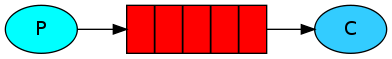
\includegraphics[scale=0.7]{../Immagini/ProducerConsumer.png}
        \caption{Comunicazione con un Producer e un Consumer}
        \label{fig:ProducerConsumer}
      \end{figure}

    \subsection{Comunicazione da Sink a Nodo}
      Il Sink produce il modello Unificato che deve essere distribuito all'intera pool di Nodi. Il paradigma di comunicazione migliore da seguire in questo caso è quello del \textit{Public\&Subscribe}, rappresentato in figura \ref{fig:PublicSubscribe}. Tramite questo paradigma il Sink comunica ad un \textit{Exchange} ( il nodo in blu della figura ) il modello e questo lo posta su ogni coda di ogni consumatore ( i Nodi ).
      \begin{figure}[h!]
        \centering
        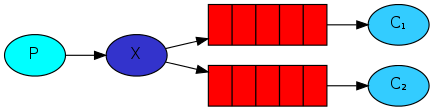
\includegraphics[scale=0.7]{../Immagini/PublicSubscribe.png}
        \caption{Comunicazione Public\&Subscribe}
        \label{fig:PublicSubscribe}
      \end{figure}

    \subsection{Registrazione di un nuovo Nodo}
      Per rendere l'architettura dinamica e flessibile è stato sviluppato un meccanismo per incrementare o diminuire il numero dei Nodi nel sistema. A questo scopo, quando un nodo vuole unirsi alla pool, deve necessariamente informare il Sink in modo tale che quest'ultimo tenga costantemente traccia del numero di Nodi presenti, necessario per l'operazione di Merging dei modelli. \newline
      La soluzione migliore in questo caso è quella di adottare un sistema di \textbf{RPC} (\textit{Remote Procedure Call}) che permette al Nodo di effettuare delle chiamate di funzioni eseguite sul Sink. Come mostrato in figura \ref{fig:RPC}, questo meccanismo si compone di 2 code:
      \begin{itemize}
        \item rpc\_queue: coda delle chiamate di funzioni
        \item reply\_to: coda dei risultati delle funzioni
      \end{itemize}
      Nel caso considerato, le funzioni disponibili sono le seguenti:
      \begin{itemize}
        \item Registration: un nodo richiede l'accesso alla pool e ottiene un identificativo univoco come risposta
        \item Leave: un nodo richiede l'uscita dalla pool specificando il proprio identificativo nella richiesta
      \end{itemize}
      \begin{figure}[h!]
        \centering
        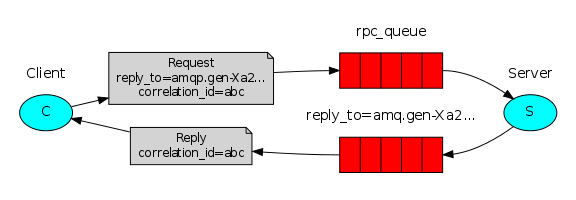
\includegraphics[scale=0.7]{../Immagini/RPC.png}
        \caption{Remote Procedure Call}
        \label{fig:RPC}
      \end{figure}


  \section{Implementazione}
    \subsection{abstract class CommunicationModelHandler}
      Il software creato si appoggia sulle Java API di \textit{RabbitMQ} che permette una facile gestione di message queueing e per via delle somiglianza tra le azioni da svolgere sia sul Sink che sui Nodi, è stata implementata una classe astratta \textit{CommunicationModelHandler} \ref{CommunicationHandler} che mantiene delle informazioni utilizzati nelle interazioni con il server di RabbitMQ e i nomi delle \textit{Queue}, comuni a tutti i nodi. Inoltre, il costruttore inizializza una connessione che il Server di RabbitMQ configurato sulla porta di default 5672 e richiama le 3 funzioni per l'inizializzazione delle strutture su cui verrano scambiati i dati:
      \begin{itemize}
        \item \textit{initRPC()}
        \item \textit{initSinkToNode()}
        \item \textit{initNodeToSink()}
      \end{itemize}
      Ognuna di queste verrà definita dal Nodo e dal Sink in modo da rispettare il proprio ruolo rispetto alla struttura in questione.
      \lstinputlisting[label={CommunicationHandler}, language=Java, caption={CommunicationModelHandler},captionpos=b]{../Codice/CommunicationModelHandler.java}

    \subsection{NodeCommunicationModelHandler}
      Questa classe è l'implementazione della \textit{CommunicationModelHandler} utilizzata su ogni Nodo per la gestione della communicazione con il Sink. Ai campi membri della super classe viene aggiunto un intero \textit{NodeID} che contiene l'identificativo del nodo. La classe definisce le funzioni astratte nel seguente modo:
      \subsubsection{initRPC()}
        Questa funzione crea un canale per comunicare con il Server RPC presente sul Sink attraverso cui si chiama la Remote Procedure per <<registrare>> il Nodo nel sistema, il quale ottiene un identificativo univoco come risposta. Tale ID è usato per distinguere i nodi tra di loro e i loro relativi modelli.
        \lstinputlisting[label={Node:initRPC}, language=Java, firstline=32, lastline=43,  caption={NodeCommunicationModelHandler.initRPC()},captionpos=b]{../Codice/NodeCommunicationModelHandler.java}

      \subsubsection{initNodeToSink()}
